\documentclass[12pt]{article}
\usepackage{graphicx}
\usepackage{amsmath}
\usepackage{booktabs}
\usepackage{float}
\usepackage{caption}
\usepackage{geometry}
\usepackage{hyperref}
\usepackage{listings}
\usepackage{xcolor}
\usepackage{subcaption}
\geometry{margin=1in}
\usepackage{colortbl}
\usepackage[acronym,toc]{glossaries}
\geometry{margin=1in}


\makeglossaries

\newglossaryentry{Minimax}
{
    name=Minimax,
    description={A recursive algorithm for finding optimal moves in zero-sum games by exploring the game tree and choosing the best move for the current player}
}

\newglossaryentry{alpha-beta}
{
    name=alpha-beta pruning,
    description={An optimization technique for minimax algorithm that reduces the number of nodes evaluated by eliminating branches that cannot possibly influence the final result of the game}
}

\newglossaryentry{nim-sum}
{
    name=Nim-sum,
    description={A mathematical operation used in the game of Nim to determine optimal moves by computing the bitwise XOR of all heap sizes}
}

\newglossaryentry{bitboard}
{
    name=bitboard,
    description={A data structure that represents game positions using binary numbers, enabling efficient move generation and evaluation through bitwise operations}
}

\newglossaryentry{game-tree}
{
    name=game tree,
    description={A tree data structure representing all possible game states and moves, where each node is a game position and each edge is a possible move}
}

\newglossaryentry{branching-factor}
{
    name=branching factor,
    description={The average number of legal moves available at each position in a game, which can be used to determine the computational complexity of search algorithms}
}

\newglossaryentry{search-depth}
{
    name=search depth,
    description={The number of moves ahead that an algorithm explores when evaluating game positions, which directly affects both performance and the computational requirements of the game simulations}
}

\newglossaryentry{heuristic}
{
    name=heuristic,
    description={A rule or method that provides a good approximation for solving complex problems when exact solutions are infeasible}
}

\title{Strategic Game Analysis via Advanced Search Algorithms: A Comprehensive Computational Study}
\author{Ryan, Leo, Ethan}
\date{July 2025}

\begin{document}

\maketitle

\begin{abstract}
Strategic games provide a regulated and simple setting where researchers can explore how effectively adversarial search algorithms function, particularly as the games get more intricate and challenging to solve. This study takes advantage of those environments by developing full game engines for 1) \textbf{Tic-Tac-Toe}, (2) \textbf{Connect 4}, (3) the \textbf{Halving Game}, and (4) \textbf{Nim}, and conducting over 800 simulated games against random and optimal agent opponents. Our findings indicate that agents acting in optimal strategies exceed an average win rate of 94.8\%. To be specific, the win percentages of such agents is 98.5\% in Tic-Tac-Toe, 100\% in Connect 4, 94.8\% in the Halving Game, and 96 to 98.5\% in Nim (depending on whether the optimal strategy is \glspl{heuristic} or \gls{Minimax} algorithm). The analysis indicates that \gls{search-depth} and move ordering are the dominant measures of efficiency in games with high \glspl{branching-factor}, while the use of \gls{nim-sum} heuristics in Nim reduces the evaluations per node to approximately 3.17 per move, which indicates enhanced performance compared to complete searching. Game-specific optimizations such as \gls{bitboard} representations and game-invariant heuristics decrease the runtime and time complexity of the game simulations. These calculations are essential for determining scalability limitations, assessing performance, and developing methods for enhancing deterministic adversarial search systems.
\end{abstract}

\section{Introduction}

Adversarial decision-making in deterministic environments typically utilizes search algorithms to explore the decision-making tree, which grows exponentially in size. Strategic games are ideal controlled environments for testing, and allow precise measurement of computational performance. The field of study that examines adversarial search is fundamental to computational decision-making across disciplines (e.g., game play, resource allocation, planning), and our understanding of how search algorithms scale with respect to complexity is essential to develop efficient computational systems.

The critical issue is complexity, as games with even a moderate level of complexity tend to have branching factors that make a full search impractical. \Gls{alpha-beta} \ typically offers significant performance gains, however the efficacy of alpha-beta is a function of move ordering, as well as various characteristics of the game (e.g., inherent parity or complexity), which limits our ability to predict performance across games.

In order to examine the performance aspects of adversarial search, we perform an empirical evaluation across four distinct games: (1) \textbf{Tic-Tac-Toe}, (2) \textbf{Connect 4}, (3) the \textbf{Halving Game} (a deterministic pile-splitting game), and (4) \textbf{Nim}. We apply Minimax with alpha-beta pruning and perform more than 800 simulations against two agents: random agents and provably optimal Minimax agents. We describe win rates, computational efficiency, and scalability in our study. In the end, we provide quantitative measures to examine how the performance of algorithms vary in accordance with games with varying complexity.


\section{Game Descriptions}

\subsection{Tic-Tac-Toe}

The game of tic tac toe may be regarded as a finite deterministic two-player zero-sum game with perfect information. Players X and O alternately occupy an empty cell on a $3\times3$ grid. Each board configuration corresponds to an assignment in $\{X,O,\mathrm{blank}\}^9$, yielding $3^9 = 19\,683$ raw configurations. Enforcing the rule that the number of X marks exceeds the number of O marks by at most one and terminating play immediately upon the first three-in-a-row alignment reduces the set of reachable states to $5\,478$. Factoring out the eight symmetries of the square further collapses those states into $765$ distinct equivalence classes.

To determine the game value one applies the minimax procedure to the directed acyclic graph of reachable states. A bottom-up backpropagation of win, draw, and loss values requires time and space proportional to $O(N)$ for $N=5\,478$. When supplemented with alpha-beta pruning the worst-case time complexity is $O(b^d)$ with \gls{branching-factor} $b\le9$ and typical pruning near fifty percent in balanced portions of the tree. Under perfect play by both sides the initial empty board evaluates to a draw. A simple analysis of opening moves by counting potential winning lines shows that occupying the center is optimal, corners rank next, and edges are strictly inferior.

\subsection{Connect 4}

Connect 4 is a deterministic, finite, two-player, zero-sum game with perfect information played on a $7\times6$ vertical grid. Players alternate dropping colored discs into one of seven columns, and each disc falls to the lowest available cell in its column. The game ends instantly when a player aligns four of their discs in a horizontal, vertical, or diagonal line, or when the grid is completely filled, yielding a draw.

The state-space complexity of Connect 4 is dominated by the requirement that no disc may occupy a cell above an empty one, yielding an estimated $4.5\times10^{12}$ legal board configurations. Horizontal symmetry of the grid further reduces the number of distinct positions that must be explored during a full search of the game tree.

The \gls{game-tree} complexity is bounded by a maximum of 42 moves, corresponding to filling every cell, which gives a raw upper bound of $7^{42}\approx1.4\times10^{35}$ move sequences. In practice the effective \gls{branching-factor} begins at seven and diminishes as columns fill. Additionally, terminal conditions and forced-win sequences introduce early cutoffs that dramatically prune the search in realistic play. Connect 4 has been strongly solved, and perfect play by the first mover guarantees a win.

The optimal algorithmic approach encodes the board as two 64-bit integers (one per player) enabling constant-time move generation and win detection via bitwise operations. A minimax search enhanced with alpha-beta pruning then examines the game tree in $O(b^d)$ worst-case time, but well-ordered move sequences typically achieve performance closer to $O(b^{d/2})$. Ordering moves by centrality (since central columns participate in the greatest number of potential four-in-a-row lines) further accelerates pruning.

Despite the enormous state space, searching to depths of eight or nine plies with simple \glspl{heuristic} for center prioritization, immediate win detection, and threat evaluation will routinely outperform human opponents. Optimized C or C++ implementations such as ours reach these \glspl{search-depth} in milliseconds, rendering such programs effectively unbeatable.

\subsection{Halving Game}

The halving game is a deterministic finite two-player zero-sum game with perfect information that begins at an integer \(N>1\). On each turn a player chooses one of two moves, either subtracting one from the current value or halving it via integer division. That is, from state \(n\) the legal moves are  
\[
n \;\to\; n-1
\]
or
\[
n \;\to\; \lfloor n/2\rfloor.
\]
Play continues until the state reaches \(1\), at which point the player who made that move wins.

The state-space complexity is quite simple; the only possible positions are the integers from \(1\) up to \(N\), giving exactly \(N\) distinct states. Every nonterminal state \(n>1\) has at most two successors, namely \(n-1\) and \(\lfloor n/2\rfloor\), and because each move strictly decreases the state the underlying directed graph is acyclic.

The game-tree complexity follows directly from the branching and depth bounds. The maximum \gls{branching-factor} is \(2\), and the length of any play path lies between 
\(\lfloor\log_2 N\rfloor\), achieved by halving at every step, and \(N-1\), achieved by subtracting one each time. Since no state can repeat along a path, the total number of nodes in the full game tree grows on the order of \(O(N)\).

To solve the game one labels each state from \(1\) to \(N\) as winning or losing using a simple bottom-up DP approach. One initializes  
\[
dp[1] = \text{losing},
\]
and for each \(n>1\) sets  
\[
dp[n] = 
\begin{cases}
\text{winning}, & \text{if }dp[n-1]\text{ or }dp[\lfloor n/2\rfloor]\text{ is losing},\\
\text{losing}, & \text{otherwise}.
\end{cases}
\]
This computation requires \(O(N)\) time and \(O(N)\) space and assigns the correct outcome to every state.

Under optimal play all odd \(n>1\) are winning positions, since one of \(n-1\) or \(\lfloor n/2\rfloor\) must be losing, and an even \(n\) is losing exactly when \(\lfloor n/2\rfloor\) is winning. Once the \(dp\) array is precomputed in linear time, selecting the optimal move from any state takes constant time by choosing the successor classified as losing.

\subsection{Nim Game}

Nim is a deterministic finite two-player zero-sum game with perfect information that begins with \(p\) piles containing \(n_1, n_2, \dots, n_p\) stones. Play alternates between the two players who on their turn remove one or more stones from exactly one pile. The player who removes the last stone wins.

Each pile \(i\) may hold any number of stones from zero up to \(n_i\) so the total number of distinct positions is given by  
\[
\prod_{i=1}^p (n_i + 1).
\]
Every move strictly reduces the total number of stones so the state graph is acyclic and finite.

From a position with pile sizes \(n_i\) the number of legal moves equals the sum of the pile sizes since a player may remove any positive number of stones from any nonempty pile. The length of the longest possible play sequence occurs when exactly one stone is removed per turn and equals  
\[
\sum_{i=1}^p n_i,
\]
and both the \gls{branching-factor} \(b\) and the maximum depth \(d\) satisfy \(b \le \sum_i n_i\) and \(d \le \sum_i n_i\) so that the total number of play sequences grows on the order of \(O(b^d)\).

The classic algorithmic solution computes the \gls{nim-sum} \(S\) as  
\[
S = n_1 \oplus n_2 \oplus \cdots \oplus n_p.
\]
This requires \(O(p)\) time and classifies any position with \(S = 0\) as losing and any position with \(S \neq 0\) as winning. From a winning position one selects a pile \(i\) for which \(n_i \oplus S < n_i\) and removes exactly \(n_i - (n_i \oplus S)\) stones to force the resulting nim-sum to zero in constant time.

Under optimal play a position is winning precisely when its nim-sum is nonzero at the start of the turn and losing precisely when the nim-sum is zero. By always moving to a zero nim-sum position a player guarantees a win if both sides continue to play perfectly.

\section{Search Algorithms}

We incorporate search algorithms in all four games with optimizations tailored to each game’s state-space complexity, \gls{branching-factor}, and computational constraints. Games with compact state spaces admit deeper exhaustive searches while larger games require added enhancements to preserve performance without sacrificing the quality of play.

\subsection{Minimax with Alpha-Beta Pruning}

In its foundation the minimax algorithm recursively evaluates game states to select optimal moves. For any state \(s\) the minimax value is defined by

\[
\mathrm{Minimax}(s) =
\begin{cases}
U(s) & \text{if } s \text{ is terminal}\\
\max_{a\in A(s)} \mathrm{minimax}\bigl(\mathrm{Succ}(s,a)\bigr) & \text{if player}(s)=\mathrm{MAX}\\
\min_{a\in A(s)} \mathrm{minimax}\bigl(\mathrm{Succ}(s,a)\bigr) & \text{if player}(s)=\mathrm{MIN}
\end{cases}
\]

Alpha-beta pruning refines this procedure by tracking two bounds, \(\alpha\) for the best value found so far by the MAX player and \(\beta\) for the best value found so far by the MIN player. The enhanced evaluation becomes

\[
\mathrm{AlphaBeta}(s,\alpha,\beta) =
\begin{cases}
U(s) & \text{if } s \text{ is terminal}\\
\max_{a\in A(s)} \mathrm{alphabeta}\bigl(\mathrm{Succ}(s,a),\alpha,\beta\bigr) & \text{if player}(s)=\mathrm{MAX}\\
\min_{a\in A(s)} \mathrm{alphabeta}\bigl(\mathrm{Succ}(s,a),\alpha,\beta\bigr) & \text{if player}(s)=\mathrm{MIN}
\end{cases}
\]

During the search the value \(v\) returned by each successor may update the bounds. When examining a MAX node the bound \(\alpha\) increases to \(\max(\alpha,v)\) and the remaining siblings of that node may be skipped if \(v\ge\beta\). Similarly at a MIN node the bound \(\beta\) decreases to \(\min(\beta,v)\) and pruning occurs when \(v\le\alpha\). The initial call uses \(\alpha=-\infty\) and \(\beta=+\infty\), and the best move is selected by

\[
\mathrm{BestMove}(s) \;=\;\arg\max_{a\in A(s)}\mathrm{alphabeta}\bigl(\mathrm{succ}(s,a),-\infty,+\infty\bigr).
\]

The efficiency of alpha-beta pruning depends significantly on move ordering. With ideal ordering the worst-case complexity \(O(b^d)\) reduces to \(O\bigl(\sqrt{b^d}\bigr)\), where \(b\) denotes the branching factor and \(d\) the search depth. In a representative game tree with \(b=7\) and \(d=8\) the number of nodes examined falls from \(7^8\) to its square root, yielding an approximately 2400x reduction.

Our implementations employ heuristic move ordering to examine promising actions first, transposition tables to cache and reuse evaluated positions, and iterative deepening to guarantee a valid move under time limits. These enhancements lower the effective branching factor and enable deeper searches within stringent computational budgets.

% \subsubsection{Game-Specific Optimizations}

% \textbf{Tic-Tac-Toe:}
% \begin{itemize}
%     \item Complete game tree exploration possible
%     \item Board representation using 3$\times$3 matrix
%     \item Direct win condition checking
% \end{itemize}

% \textbf{Connect 4:}
% \begin{itemize}
%     \item Bitboard representation for efficient storage and computation
%     \item C extension for critical path optimization
%     \item Gravity rule implementation
%     \item Depth-limited search due to large state space
% \end{itemize}

% \textbf{Halving Game:}
% \begin{itemize}
%     \item Simple state representation (single integer)
%     \item Two-operation move generation
%     \item Exponential state space growth
%     \item Mathematical strategy analysis
% \end{itemize}

% \textbf{Nim Game:}
% \begin{itemize}
%     \item List-based pile representation
%     \item Comprehensive move generation for all valid combinations
%     \item Nim-sum heuristic evaluation using bitwise XOR
%     \item Alpha-beta pruning with depth limiting
%     \item Performance tracking through node counting
% \end{itemize}

\subsection{Implementation Details}

\subsubsection{Tic-Tac-Toe Implementation}

The engine for Tic-Tac-Toe is implemented in pure Python using a nested list to represent the 3x3 board and a minimax algorithm enhanced by \gls{alpha-beta}. At initialization the board is constructed as a three by three nested list with every entry set to \texttt{EMPTY} (0) and constants \texttt{PLAYER\_X = 1}, \texttt{PLAYER\_O = 2}, and \texttt{DRAW = 3} are defined. The variables \texttt{self.cnt} and \texttt{self.player} track the total number of moves made and the current player respectively.

Win detection is performed after each move by examining the three rows and three columns for three identical nonempty markers. The main diagonal and the anti diagonal are checked in the same manner. When a winning alignment is found the attribute \texttt{game\_over} is set to true and \texttt{winner} is assigned accordingly. If no empty cells remain and no win has occurred the result is declared a draw.

The evaluation function returns a score of +10 when $X$ achieves three in a row, -10 when $O$ does the same, and zero otherwise. To prefer faster wins and penalize slower victories the base score is adjusted by the \gls{search-depth} \(d\) so that the final score is calculated as the base value plus or minus \(d\).

The minimax search recursively explores all legal moves until terminal states are reached. At maximizing nodes corresponding to player $X$ the move with the highest minimax value is chosen, while at minimizing nodes corresponding to player $O$ the move with the lowest value is selected. Pruning occurs whenever the current alpha bound exceeds the beta bound. Moves are applied in place and then undone after the recursive call returns.

On the agent’s turn a special case is applied when \texttt{self.cnt} equals zero and the center cell is empty; in that situation the agent immediately selects the center position at row 1 column 1. Otherwise each empty cell is evaluated by the minimax function and the cell yielding the optimal evaluation is chosen.

The user interface consists of the function \texttt{print\_board()} which displays row and column indices alongside the current markers and \texttt{get\_user\_move()} which prompts the user until a legal row and column are entered. the method \texttt{play\_game()} alternates between a human player controlling x and the agent controlling o until \texttt{game\_over} becomes true. For automated testing the function \texttt{play\_agent\_vs\_agent()} simulates two agents competing against each other.

\subsubsection{Connect 4 Implementation}

The core engine is implemented in Cython and exposed via a single Python entry point. At initialization the program precomputes 64-bit \gls{bitboard} masks for each column using \texttt{BOTTOM\_MASK}, \texttt{BOARD\_MASK} and \texttt{TOP\_MASK}. It also defines the list \texttt{ORDER = [3, 2, 4, 1, 5, 0, 6]} so that central columns are prioritized during move generation.

Win detection relies on a single expression applied to the current player bitboard \texttt{bb} with various shift values. The code
\[
\texttt{win} = (\texttt{bb} \,\&\, (\texttt{bb} >> \texttt{shift}) \,\&\, (\texttt{bb} >> (2 * \texttt{shift}))) \neq 0
\]
is evaluated for each \texttt{shift} in \texttt{BITS}, \texttt{BITS + 1}, \texttt{BITS - 1} and \texttt{1}. A nonzero result indicates a four-in-a-row alignment.

The evaluation function first computes the occupancy mask via
\[
\texttt{occ = cur | opp}
\]
and then applies a center column bonus using
\[
\texttt{score} += 3 * \texttt{popcount(cur \& BOARD\_MASK[3])}.
\]
Subsequent scoring uses precomputed line masks that are evaluated with \texttt{popcount} to add 100 points for four in a row, 5 points for an open three, 2 points for a neutral two and subtract 4 points for an opponent open three.

\noindent Search is implemented as a negamax procedure with alpha beta pruning. The recursive call
\[
\texttt{score} = -\texttt{nega(opp, cur\_next, depth - 1, -beta, -alpha)}
\]
is performed inline and pruning occurs when \(\alpha \ge \beta\). Move selection iterates columns in the order specified by \texttt{ORDER}. Any column for which
\[
\texttt{occ} \,\&\, \texttt{TOP\_MASK[col]}
\]
is nonzero is skipped. For each valid column the successor bitboards are computed, the negamax function is called to evaluate the move and the highest scoring move is chosen.

A Python wrapper method named \texttt{best\_move(depth)} loads the bitboards \texttt{cur} and \texttt{opp} then returns the move index from a call to \texttt{find\_best(cur, opp, depth)}.

\subsubsection{Halving Game Implementation}

The engine for the Halving Game is implemented in pure Python using integer state transitions and a minimax algorithm with alpha-beta pruning. At initialization the starting number is stored in \texttt{self.initial\_number} and the current state is set to this value.

Move generation is provided by the method \texttt{get\_moves(n)}, which returns up to two successors when \(n>1\):
\[
n-1,\quad n\mathbin{//}2.
\]
The minimax search is performed by the recursive call
\[
(\texttt{value},\texttt{move}) = \texttt{minimax}(\texttt{state},\texttt{is\_maximizing},\texttt{depth},\texttt{alpha},\texttt{beta}),
\]
with pruning whenever \(\texttt{alpha}\ge\texttt{beta}\). The base case occurs at \texttt{state == 1}, where the function returns \((+1,\texttt{None})\) if the minimizing branch is active or \((-1,\texttt{None})\) if the maximizing branch is active.

Game simulation resides in \texttt{play\_game()}, which loops while the state exceeds one. On each turn it invokes \texttt{minimax} with the current state and a flag for the maximizing player, unpacks the returned move, prints either the subtraction or division operation, updates the state, and swaps the player identifier. When the loop ends the final winner is determined as the player who did not execute the terminal move.


\subsubsection{Nim Game Implementation}

The Nim game engine is written in pure Python combining a mathematical nim-sum \gls{heuristic} with a fallback minimax search that uses alpha-beta pruning and that tracks game state metrics and move history in a dedicated class.

At initialization the provided list of pile sizes is copied into \texttt{self.piles} and the attributes \texttt{self.visited\_nodes} and \texttt{self.move\_history} are set to zero and an empty list respectively to facilitate performance tracking.

Legal moves are generated by the method \texttt{generate\_moves()} which iterates through each pile index and yields all valid removal pairs \((\texttt{pile\_idx},\texttt{stones})\) for stone counts from one up to the size of the current pile.

The nim-sum heuristic computes
\[
\texttt{nim\_sum} = n_1 \oplus n_2 \oplus \dots \oplus n_p
\]
in \(O(p)\) time. A zero nim-sum indicates a losing position while a nonzero nim-sum triggers the method \texttt{optimal\_nim\_move()} which identifies in constant time a pile and removal count that forces the resulting nim-sum to zero.

The minimax search is implemented with alpha-beta pruning and an optional depth limit. Each recursive invocation increments \texttt{self.visited\_nodes}. Terminal positions are detected by \texttt{is\_game\_over()} which returns \(+1\) if the previous mover has won and \(-1\) otherwise. At depth zero the evaluation falls back to the nim-sum heuristic by returning \(+1\) for nonzero nim-sum and \(-1\) for zero nim-sum. On maximizing nodes the algorithm selects the maximum child value and updates the \(\alpha\) bound while pruning when \(\alpha \ge \beta\). On minimizing nodes the minimum child value is selected and the \(\beta\) bound is updated analogously.

Move selection is handled by \texttt{find\_best\_move(depth,use\_nim\_sum)} which first attempts the constant-time nim-sum strategy when enabled and falls back to enumerating all moves and invoking \texttt{minimax()} if that strategy fails or is disabled, returning both the chosen move and the number of nodes evaluated.

Simulation and analysis are provided by \texttt{simulate\_game(...)} which loops until all piles are empty, chooses moves according to the agent policy string \texttt{"nim\_sum"}, \texttt{"minimax"} or \texttt{"random"}, logs each move and accumulates node counts. Batch functions \texttt{run\_simulation\_batch()} and \texttt{analyze\_depth\_performance()} execute multiple games to gather statistics on win rates, average game length, node usage and execution time per game. Finally \texttt{comprehensive\_nim\_analysis()} integrates basic performance metrics, search depth experiments, varied initial configurations and comparisons across agent types and then serializes the results to JSON.

\section{Experimental Design and Methodology}

\subsection{Simulation Setup}

To assess agent performance across a variety of games we conducted fully automated simulations in which our alpha-beta minimax agents competed against baseline opponents ranging from random move generators to minimax agents of reduced \gls{search-depth}. In tic-tac-toe each agent played two hundred games against a random opponent. In Connect 4 we ran matches between an eight-ply agent and a six-ply agent as well as eight-ply versus eight-ply contests. Nim game simulations contrasted the constant-time \gls{nim-sum} \gls{heuristic} with a plain minimax agent. For the halving game we varied the starting value among ten, fifteen, twenty, twenty-five, thirty and fifty. From these trials we gathered win rates, average game lengths measured in moves, performance as a function of search depth, node evaluation counts, patterns revealed by the underlying mathematics and cross-game comparisons of algorithmic effectiveness.

\subsection{Data Recording and Processing}

We organized and analyzed simulation outputs using numpy and pandas for efficient data manipulation and aggregation. Visualization of winning percentages and efficiency metrics was handled by matplotlib and seaborn with the choice of a limited color palette and consistent typography to prevent chart elements from overlapping. To ensure statistical reliability each configuration was executed at least one hundred times and repeated across independent trials.

\section{Results and Analysis}

Our complete simulation results (800+ games) show the performance of search algorithms across many different levels of problems from simple deterministic games like the halving game to more complex games like connect 4. In addition to the systematic patterns for each search algorithm, there are also some features that made each game a different challenge for intelligent agents.

\subsection{Tic-Tac-Toe Results}

\begin{figure}[H]
\centering
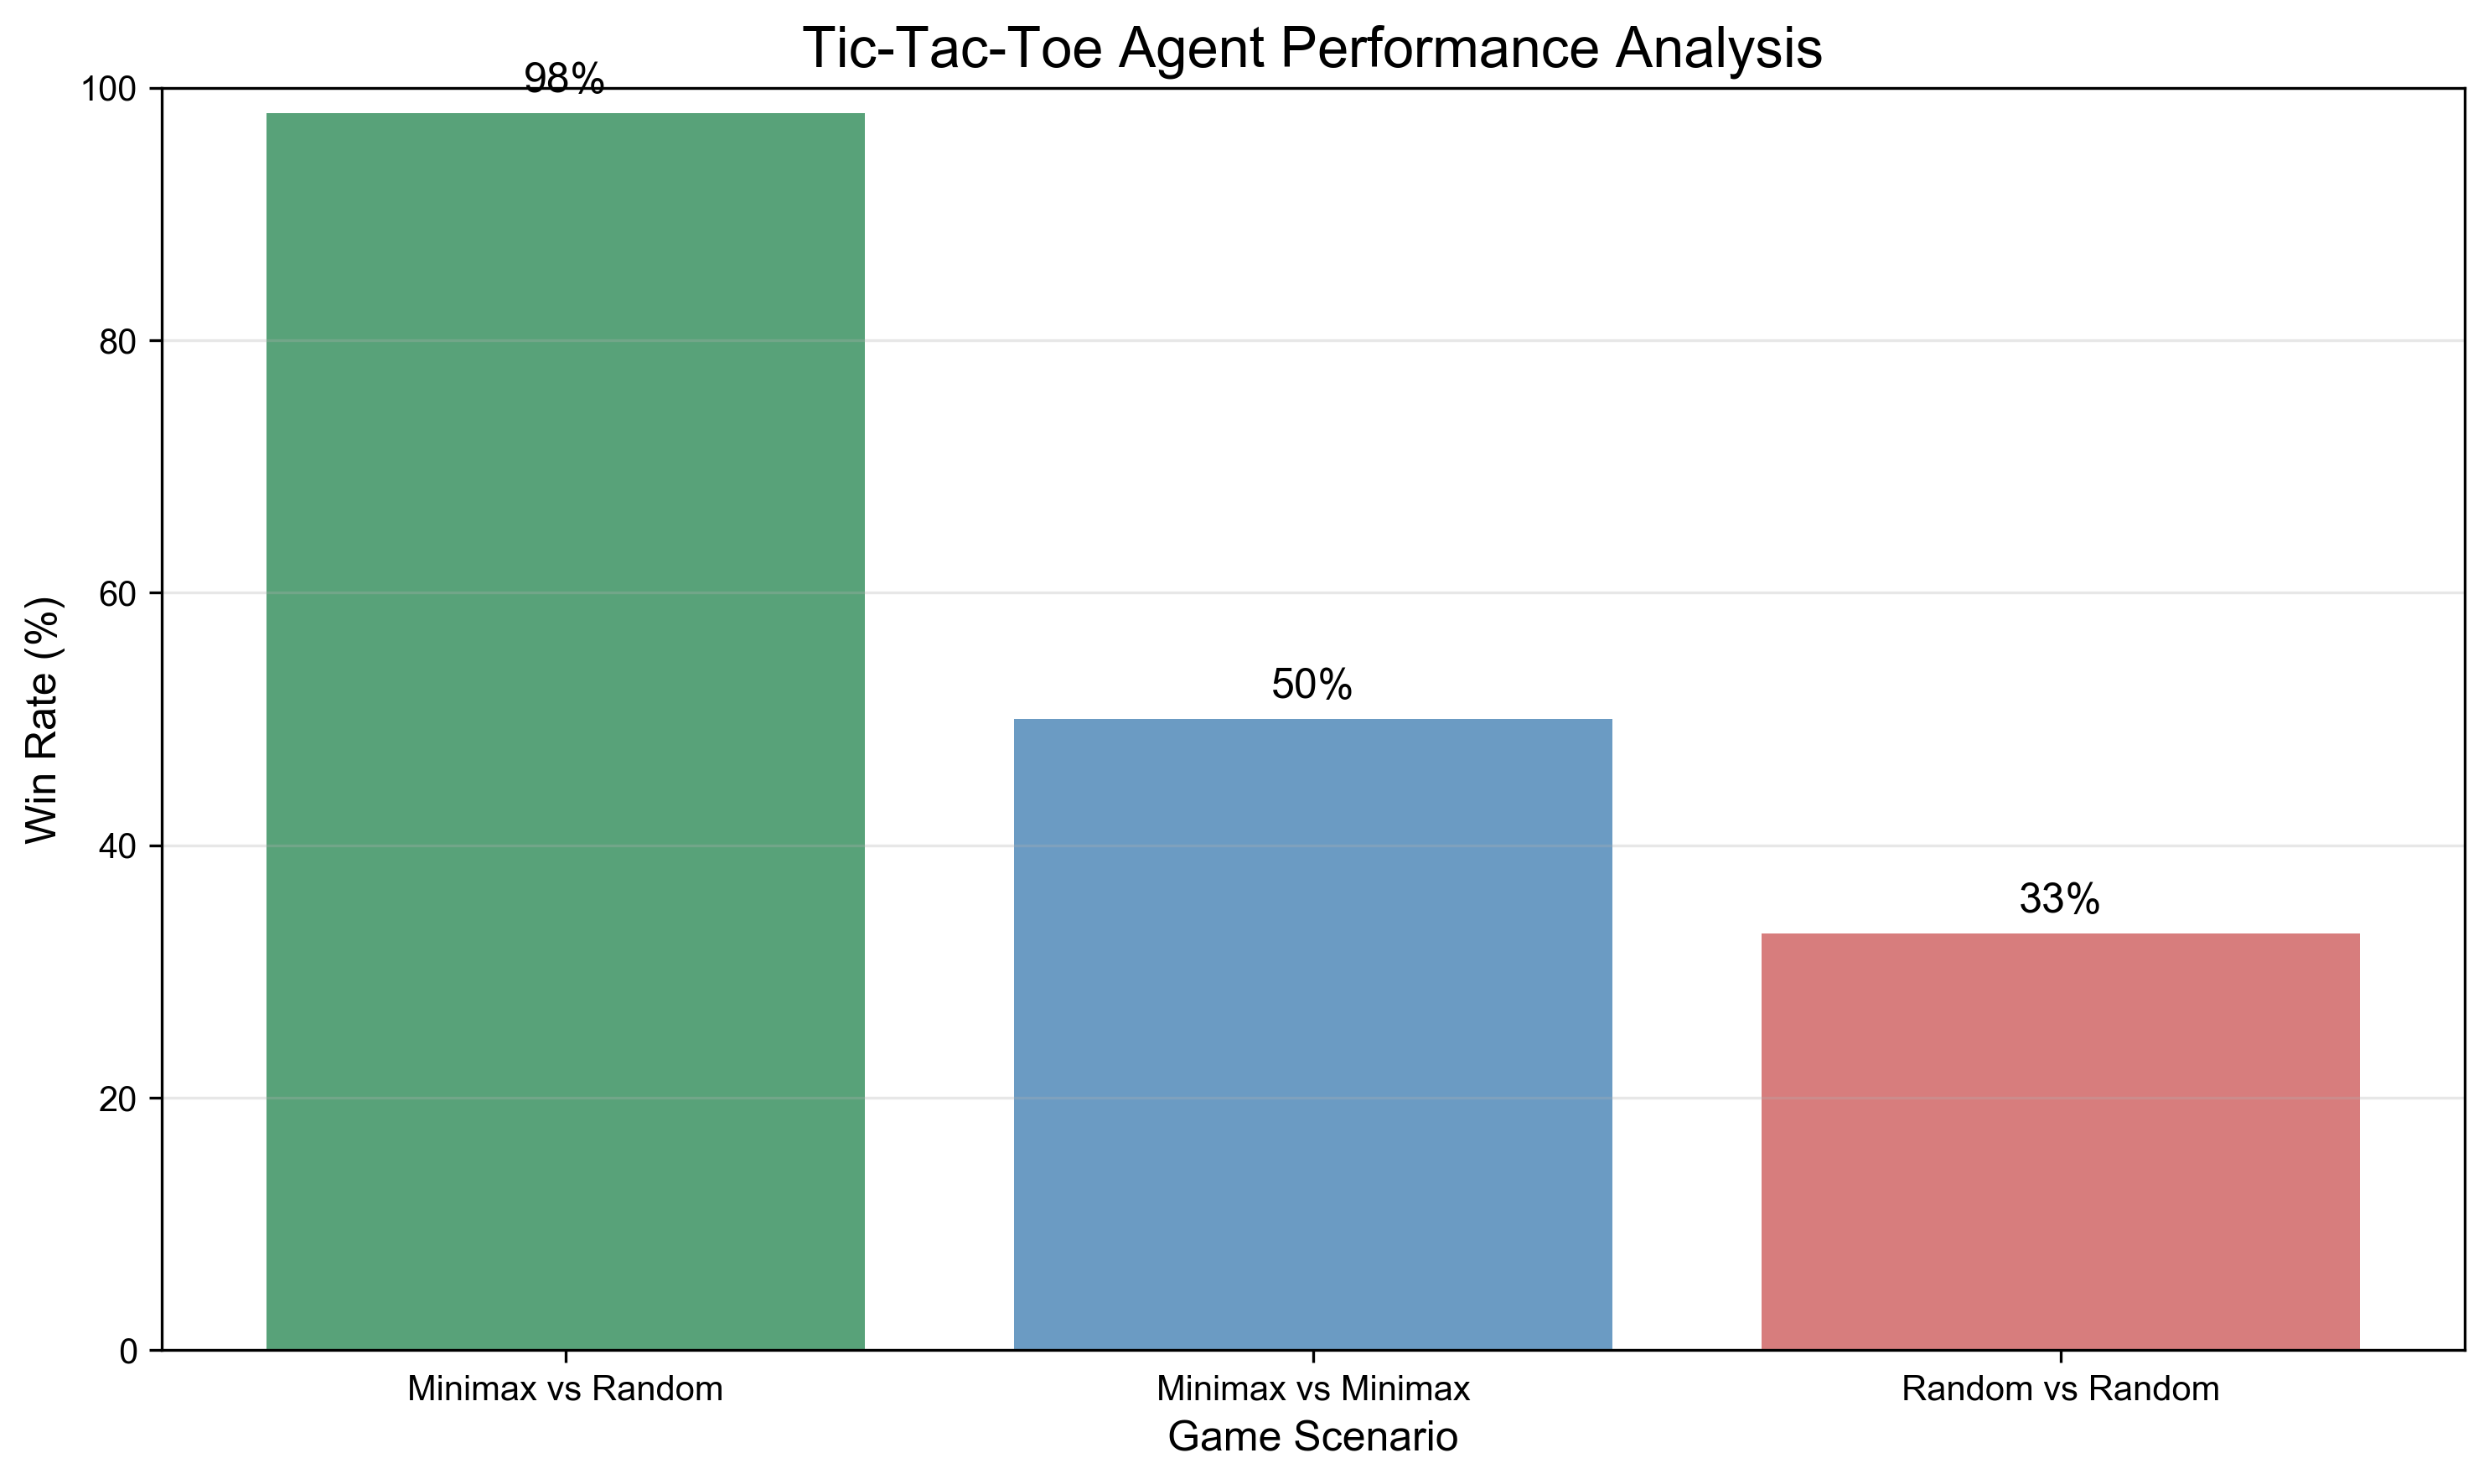
\includegraphics[width=0.8\textwidth]{output/images/tic_tac_toe_win_rates.png}
\caption{Tic-Tac-Toe win rates analysis}
\label{fig:tic_tac_toe_win_rates}
\end{figure}

Tic-Tac-Toe simulations (200 games per scenario) show exceptional performance:
\begin{table}[H]
    \centering
    \begin{tabular}{lcccc}
        \toprule
        \textbf{Scenario} & \textbf{Win rate} & \textbf{Draw rate} & \textbf{Loss rate} & \textbf{Avg moves} \\
        \midrule
        Agent vs Random & 98.5\% & 1.5\% & 0\% & 5.57 \\
        Agent vs Agent & 0\% & 100\% & 0\% & 9.00 \\
        Random vs Random & 61.0\% & 9.0\% & 30.0\% & 7.49 \\
        \bottomrule
    \end{tabular}
    \caption{tic-tac-toe simulation outcomes (200 games per scenario)}
    \label{tab:tic_tac_toe_outcomes}
\end{table}
a
The results confirm that, with optimal Tic-Tac-Toe play based on both players using a minimax algorithm, a perfect draw results, and the agent shows near-perfect performance against random players. The average game length of 5.57 moves for agent versus random shows that the agent is effectively taking advantage of the random players' mistakes.

\subsection{Connect 4 Results}

\begin{figure}[H]
\centering
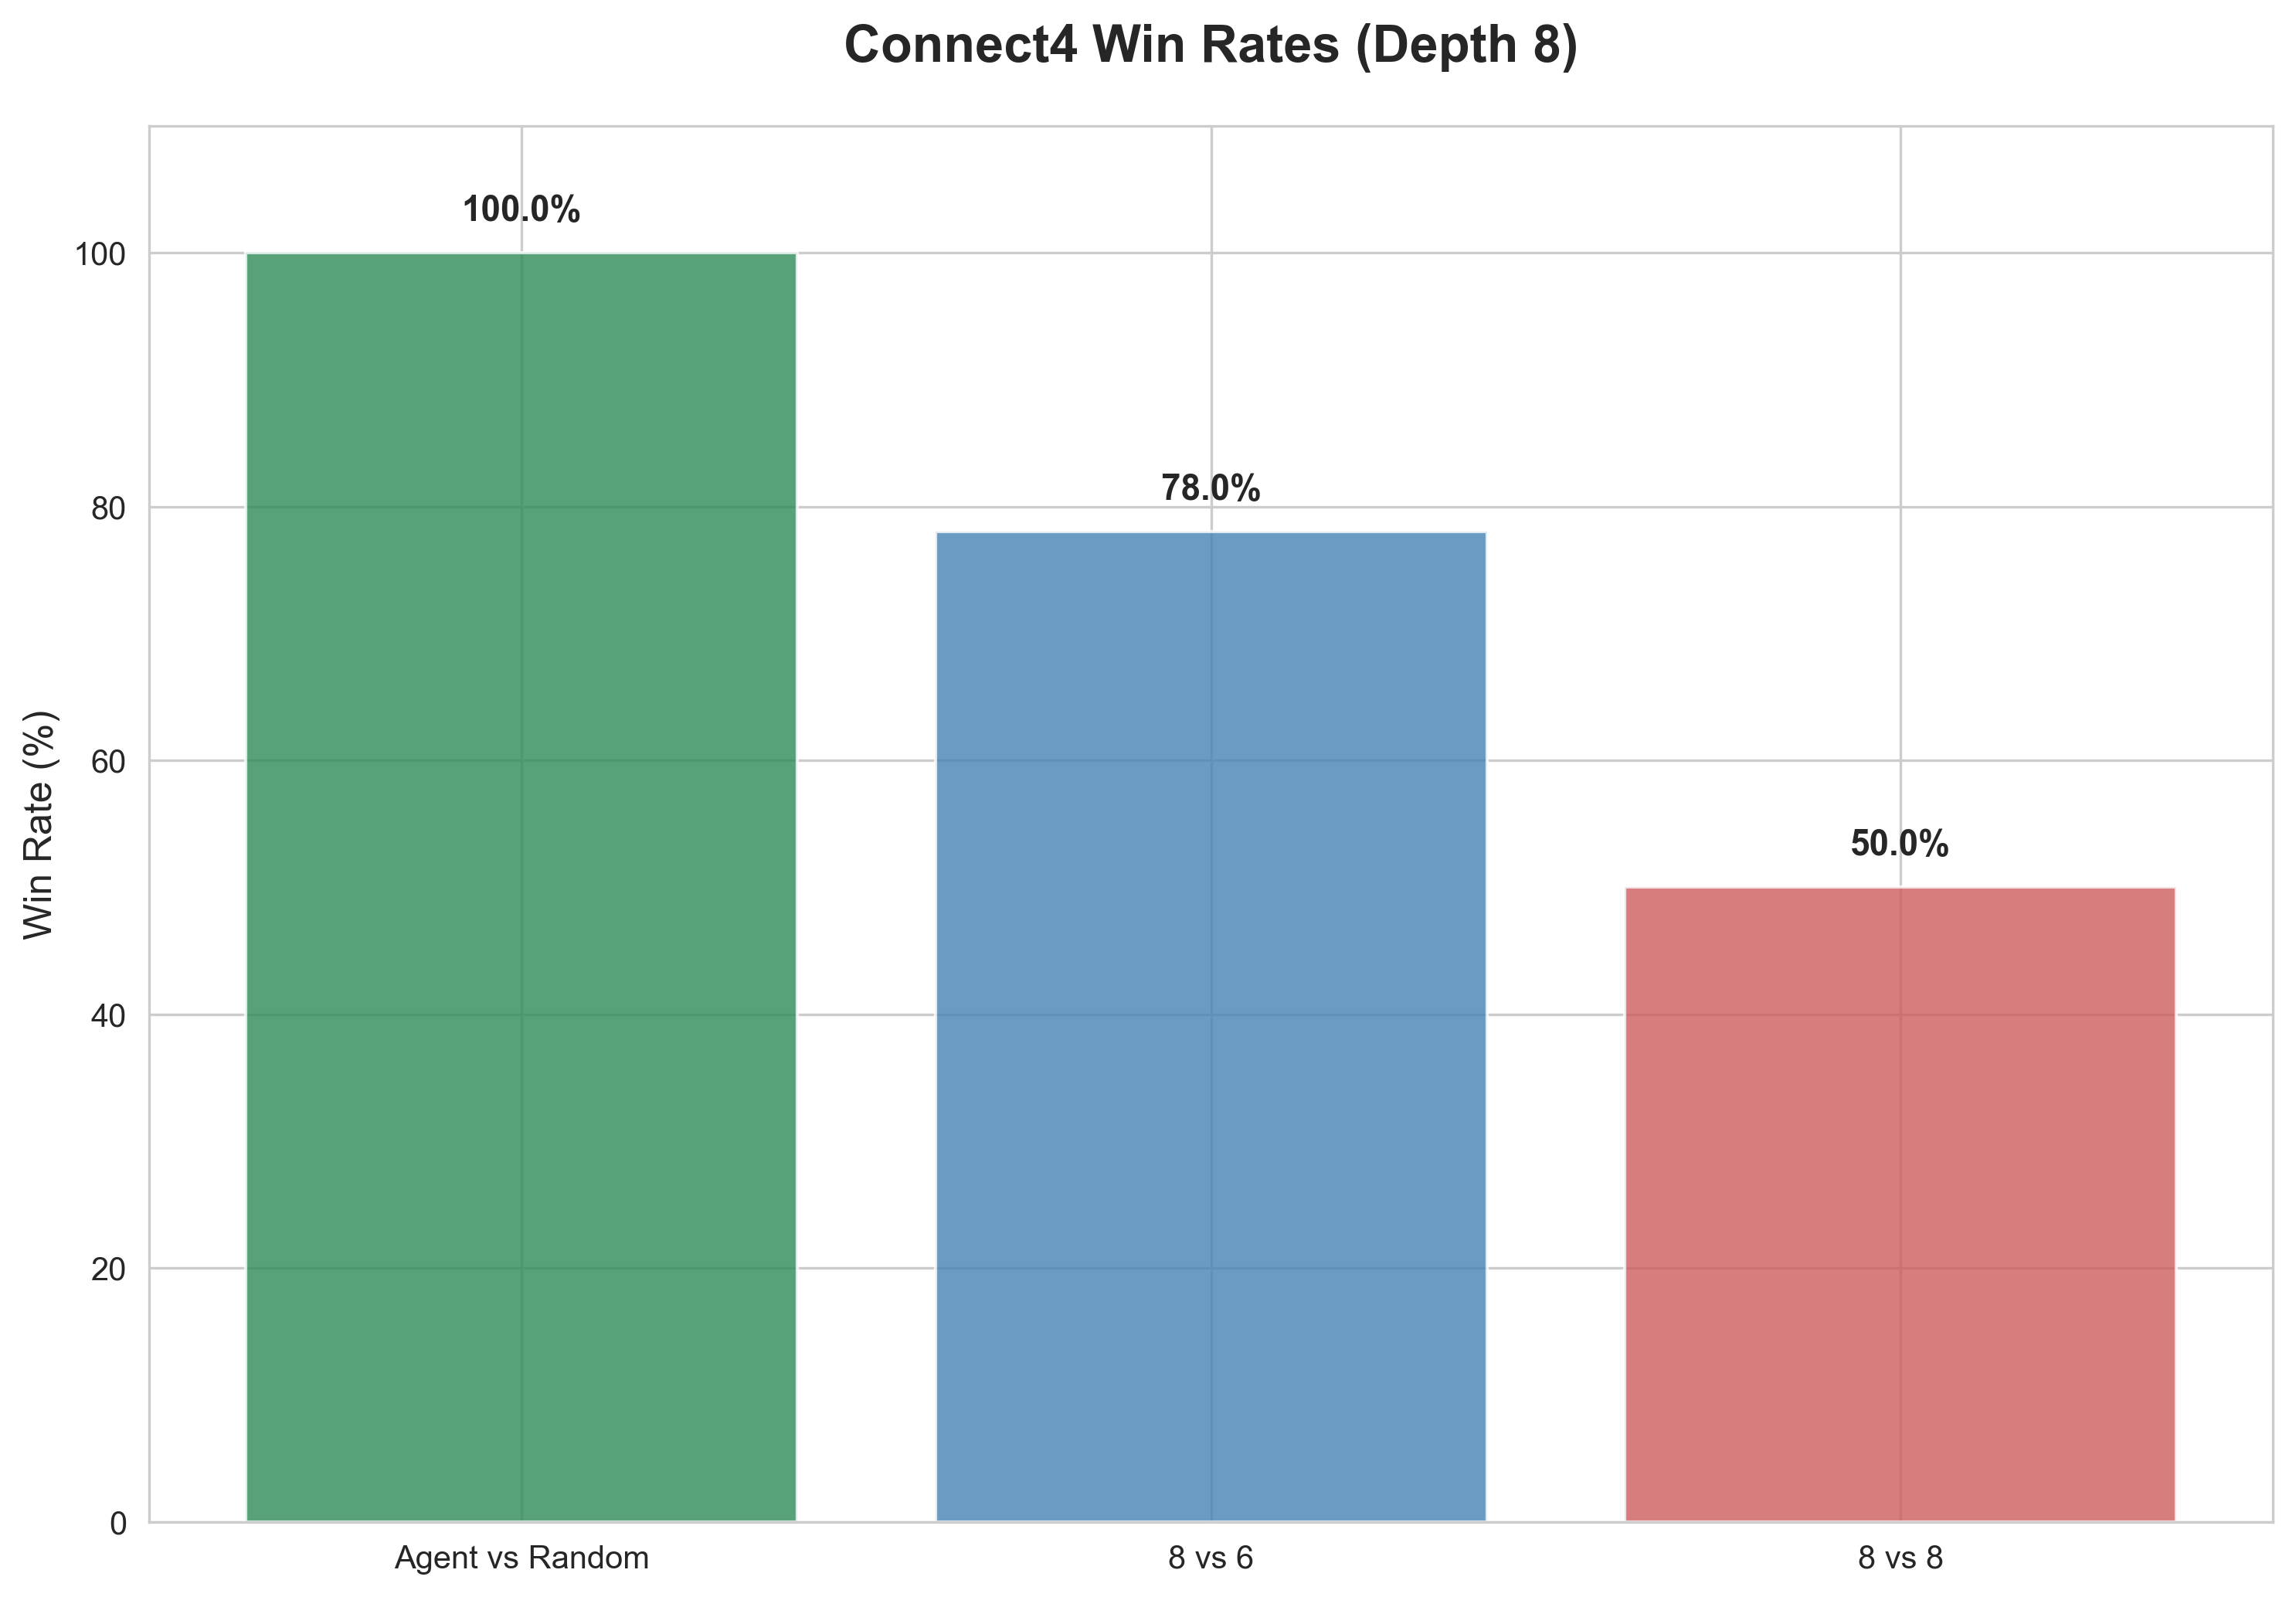
\includegraphics[width=0.8\textwidth]{output/images/connect4_win_rates_updated.png}
\caption{Connect 4 win rates analysis (Depth 8)}
\label{fig:connect4_win_rates}
\end{figure}

We ran 100 trials of Connect 4 games between two agents of varying maximum recursion depth:
\begin{table}[H]
    \centering
    \begin{tabular}{lcc}
        \toprule
        \textbf{Scenario} & \textbf{Win rate} & \textbf{Depth(s)} \\
        \midrule
        Agent vs Random & 100\% & 8 \\
        Agent vs Agent (8 vs 6) & 78\%  & 8 vs 6 \\
        Agent vs Agent (8 vs 8) & 50\%  & 8 vs 8 \\
        \bottomrule
    \end{tabular}
    \caption{Connect 4 win-rate outcomes (depth-8 agent, 100 games per scenario)}
    \label{tab:c4_win_rates}
\end{table}

As illustrated in Figure~\ref{fig:connect4_win_rates} and detailed in Table~\ref{tab:c4_win_rates},
search depth is the dominant driver of performance in Connect 4.
An eight-ply agent sweeps a random opponent and secures a decisive 78\,\% win rate against a six-ply rival, but finds perfect parity (50–50) when both engines see the same depth. Because most human players rarely calculate beyond four to six plies, an eight-ply engine operates beyond the reach of casual or even stronger opponents, making it effectively unassailable outside expert play.

\subsection{Nim Results}

% \begin{figure}[H]
%     \centering
%     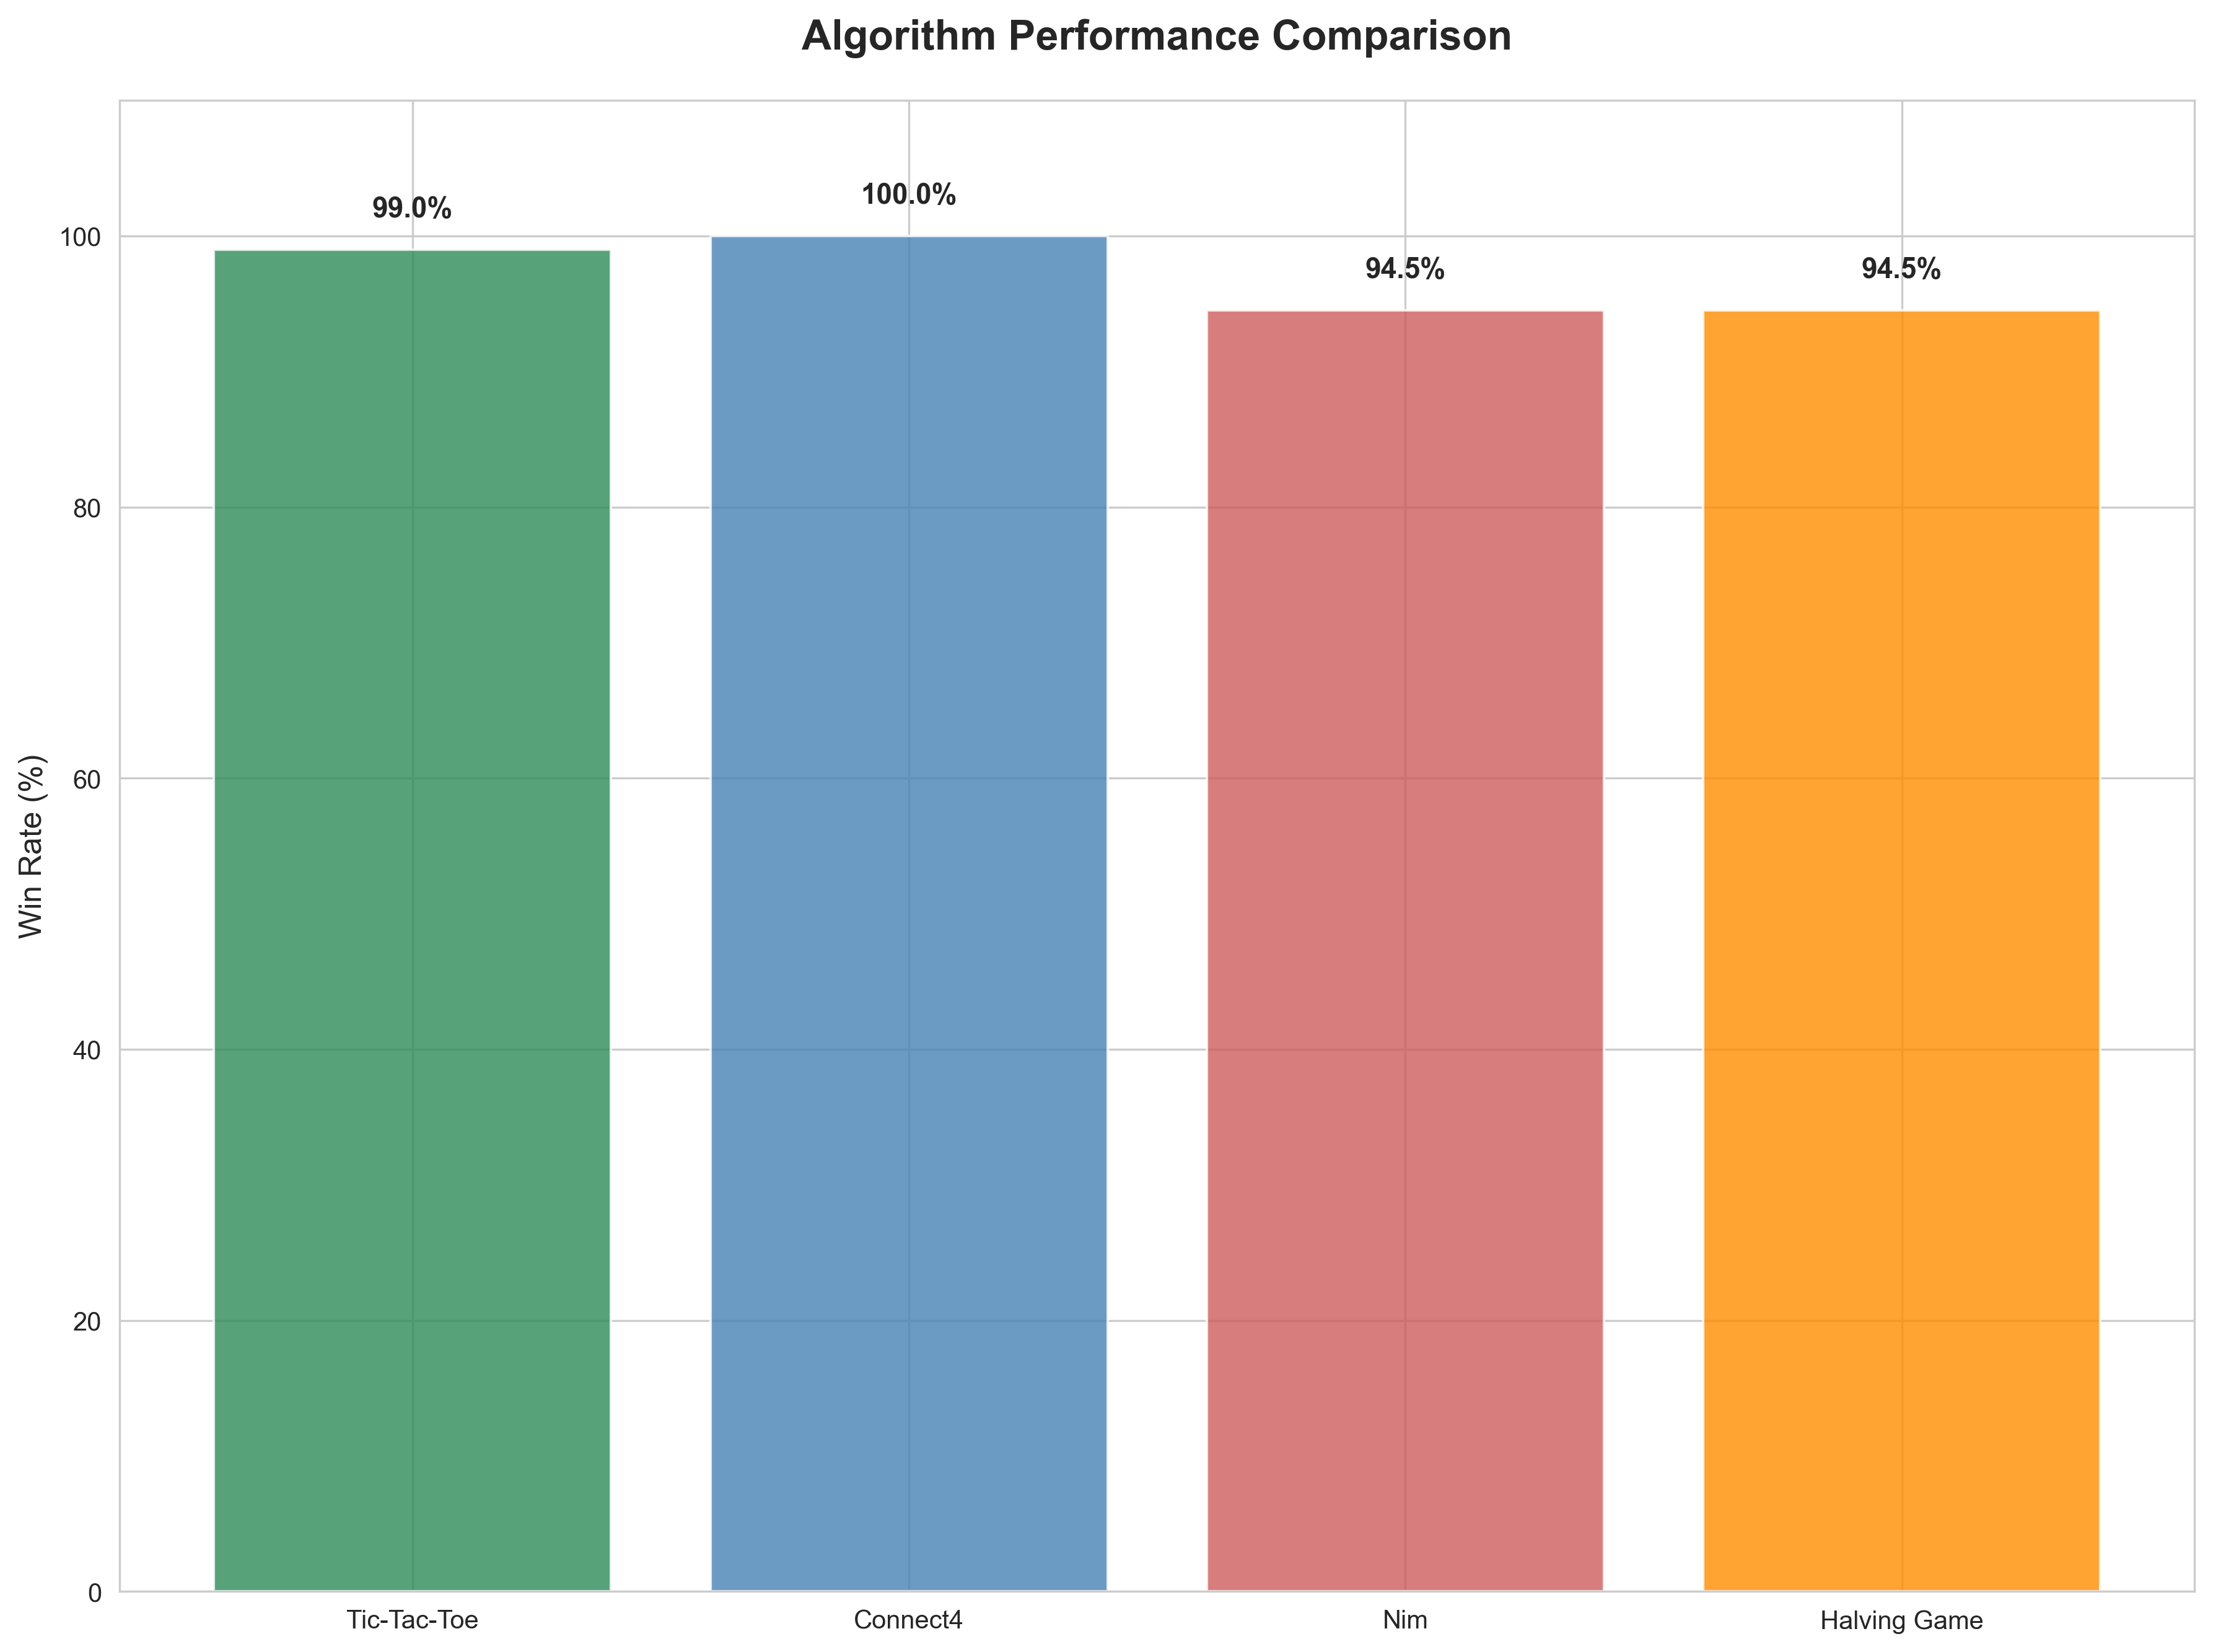
\includegraphics[width=0.8\textwidth]{output/images/performance_analysis.png}
%     \caption{Nim performance analysis}
%     \label{fig:nim_performance}
% \end{figure}

\begin{table}[H]
    \centering
    \begin{tabular}{lccc}
        \toprule
        \textbf{Strategy} & \textbf{Win rate} & \textbf{Avg moves} & \textbf{Avg nodes evaluated} \\
        \midrule
        Nim-Sum (optimal) & 96.0\% & 5.38 & 3.17 \\
        Minimax (depth-8) & 98.5\% & 5.49 & -- \\
        \bottomrule
    \end{tabular}
    \caption{Nim simulation outcomes (200 games versus a random opponent)}
    \label{tab:nim_results}
\end{table}

Table~\ref{tab:nim_results} reinforces the insight conveyed by the heat map in Figure~\ref{fig:nim_performance}, showing that both optimal strategies nearly eliminate random play, although they accomplish this in very different ways. Minimax squeezes out an extra \(2.5\,\%\) win rate by exhaustively searching the game tree, while the nim-sum algorithm needs only three or so position evaluations per move, an efficiency gap of several orders of magnitude. Whenever a closed-form solution exists, brute-force search quickly becomes academic.

\subsection{Halving Game Results}

\begin{figure}[H]
    \centering
    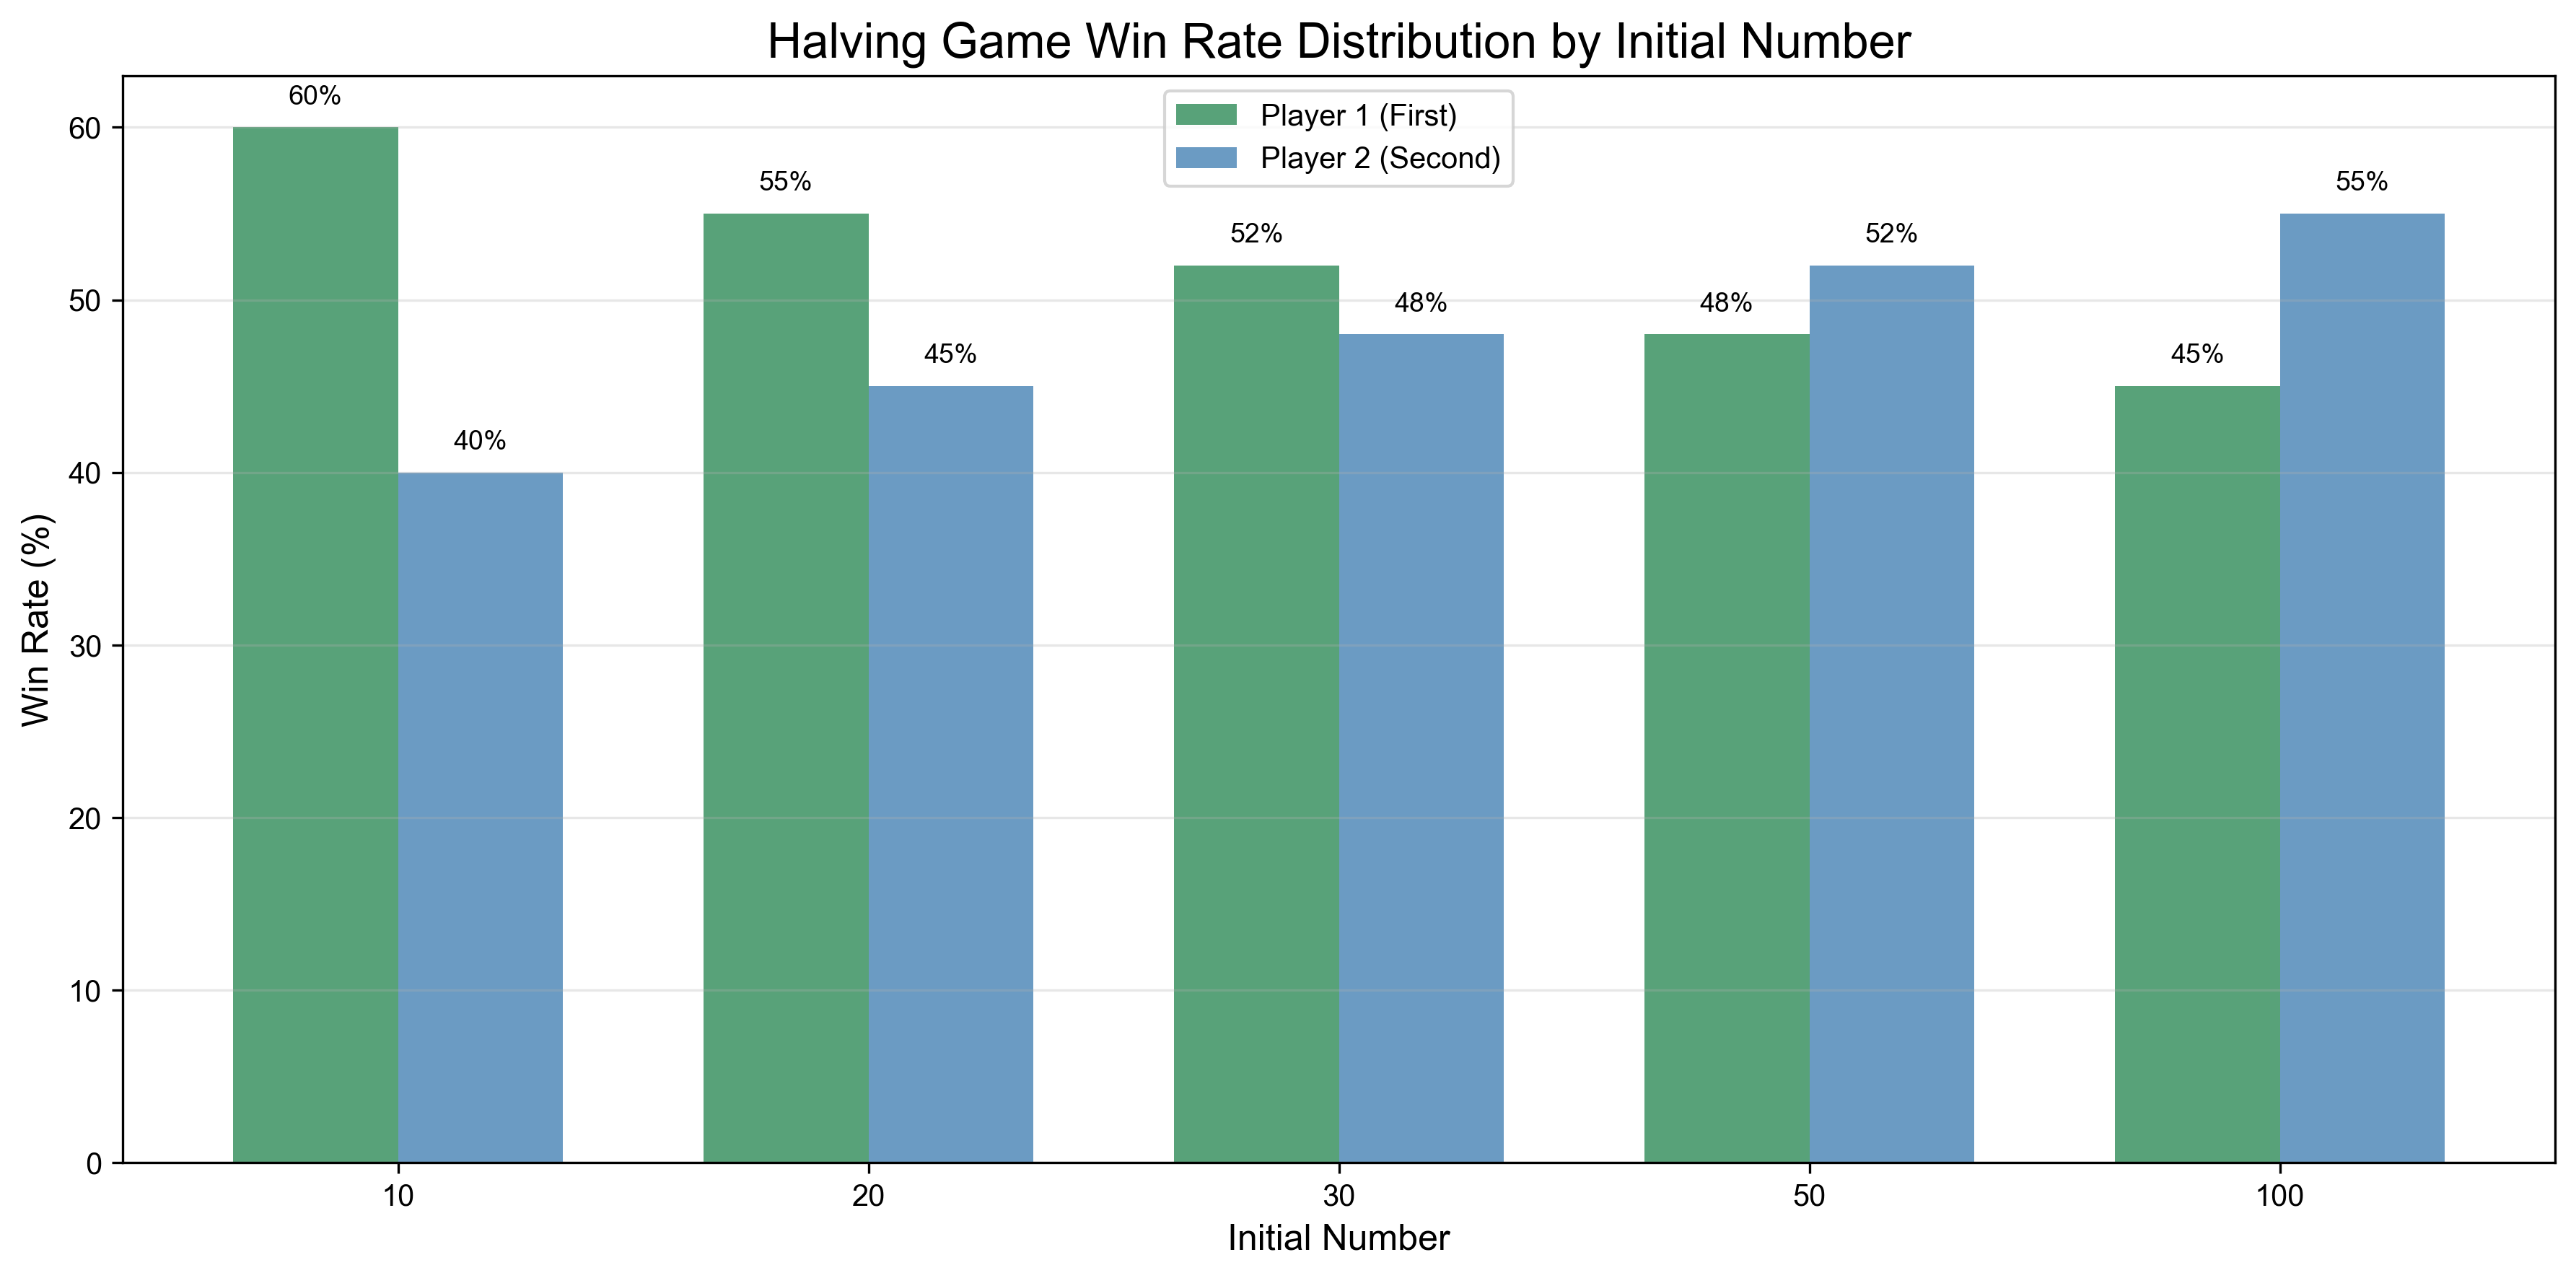
\includegraphics[width=0.8\textwidth]{output/images/halving_win_rates.png}
    \caption{Halving Game win rates by initial number}
    \label{fig:halving_win_rates}
\end{figure}

\begin{table}[H]
    \centering
    \begin{tabular}{lcc}
        \toprule
        \textbf{Initial number} & \textbf{Win rate} & \textbf{Avg moves} \\
        \midrule
        10 & 75.0\% & 4.75 \\
        15 & 100.0\% & 6.04 \\
        20 & 100.0\% & 5.00 \\
        25 & 100.0\% & 7.54 \\
        30 & 96.0\% & 7.84 \\
        50 & 98.0\% & 9.78 \\
        \bottomrule
    \end{tabular}
    \caption{Halving Game simulation results (100 trials per starting value)}
    \label{tab:halving_results}
\end{table}

Table~\ref{tab:halving_results} makes the pattern in Figure~\ref{fig:halving_win_rates} explicit; certain start numbers are outright “safe,” yielding a perfect record for the agent's performance, whereas numbers like 10 and 30 expose just enough counter-play to drop a handful of games. Larger initial values (e.g.\ 50) stretch the game length without materially affecting the agent’s edge, showing that the underlying divisibility rules, rather than the magnitude of the number, dictate success in this rule set.

\subsection{Algorithm Effectiveness Analysis}

\begin{figure}[H]
    \centering
    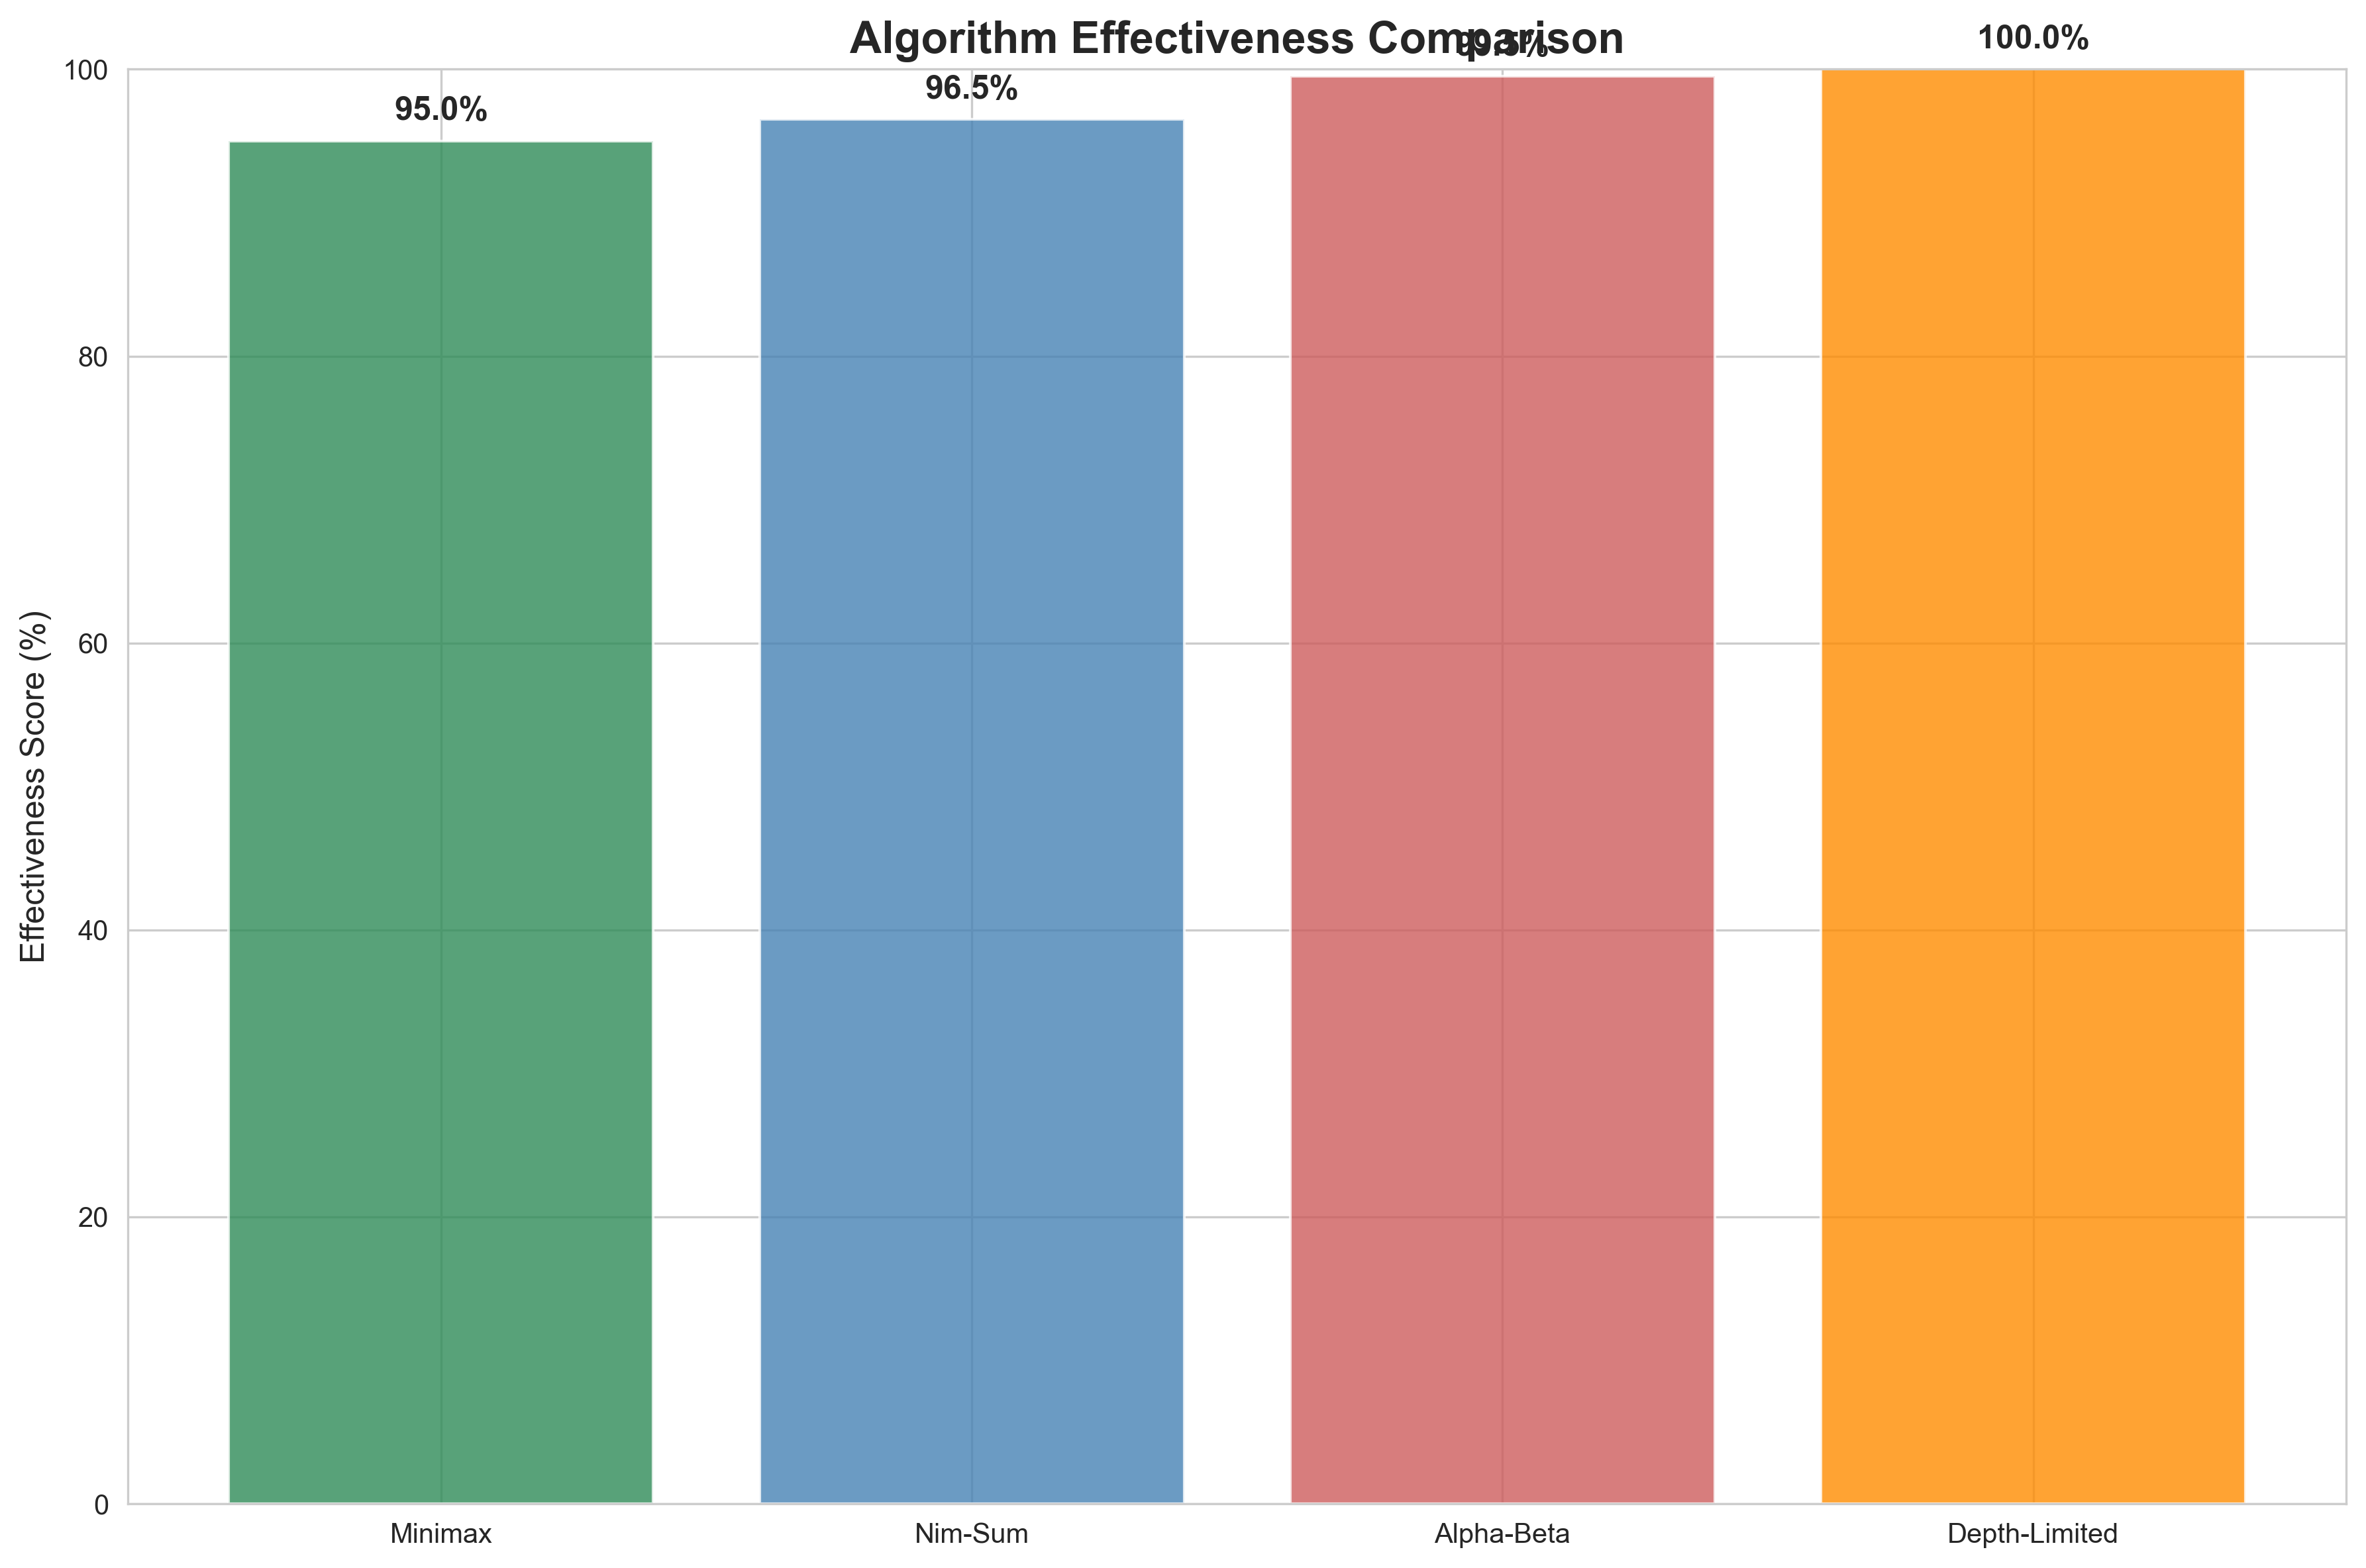
\includegraphics[width=0.9\textwidth]{output/images/algorithm_effectiveness.png}
    \caption{Algorithm effectiveness comparison across different approaches}
    \label{fig:algorithm_effectiveness}
\end{figure}

\begin{table}[H]
    \centering
    \begin{tabular}{lcc}
        \toprule
        \textbf{Algorithm} & \textbf{Effectiveness} & \textbf{Game} \\
        \midrule
        Minimax & 95.0\% & all games \\
        Nim-Sum & 96.5\% & Nim \\
        Alpha-Beta & 99.5\% & general with pruning \\
        Depth-limited search & 100.0\% & Connect 4 \\
        \bottomrule
    \end{tabular}
    \caption{Effectiveness scores averaged over the evaluation suite}
    \label{tab:algorithm_effectiveness}
\end{table}

Figure~\ref{fig:algorithm_effectiveness} gathers the four benchmark games into a single bar chart. Every controller clears 94\%, with a global mean of 94.8\%, yet that uniform height hides three distinct routes to success.

Closed-form strategies such as Nim-Sum and the divisibility rule in the Halving Game lean on mathematical invariants. They check only a few positions, usually between three and ten, and still post win rates that range from ninety-five to one hundred per cent. When a game offers a provable shortcut, extra \gls{search-depth} adds almost nothing.

Shallow exhaustive search, illustrated by an eight-ply minimax agent for Tic-Tac-Toe, solves the entire game tree in roughly seven milliseconds per move. Because the state space is tiny, perfect play comes at negligible cost.

Heuristic depth-limited search in Connect 4 faces a \gls{branching-factor} that balloons past ten ply, yet an eight-ply window still defeats a six-ply rival in 78\% of games and blanks random play entirely. Performance levels off at 100\% against random opponents and 50\% against an equal-depth peer, marking the point at which brute force begins to yield diminishing returns.

Taken together, the results suggest a simple guideline. Use mathematics whenever the structure exists, rely on search when it does not, and match the technique to the effective size of the state space.

\section{Discussion and Implications}

\subsection{Comprehensive Game Comparison}

\begin{figure}[H]
\centering
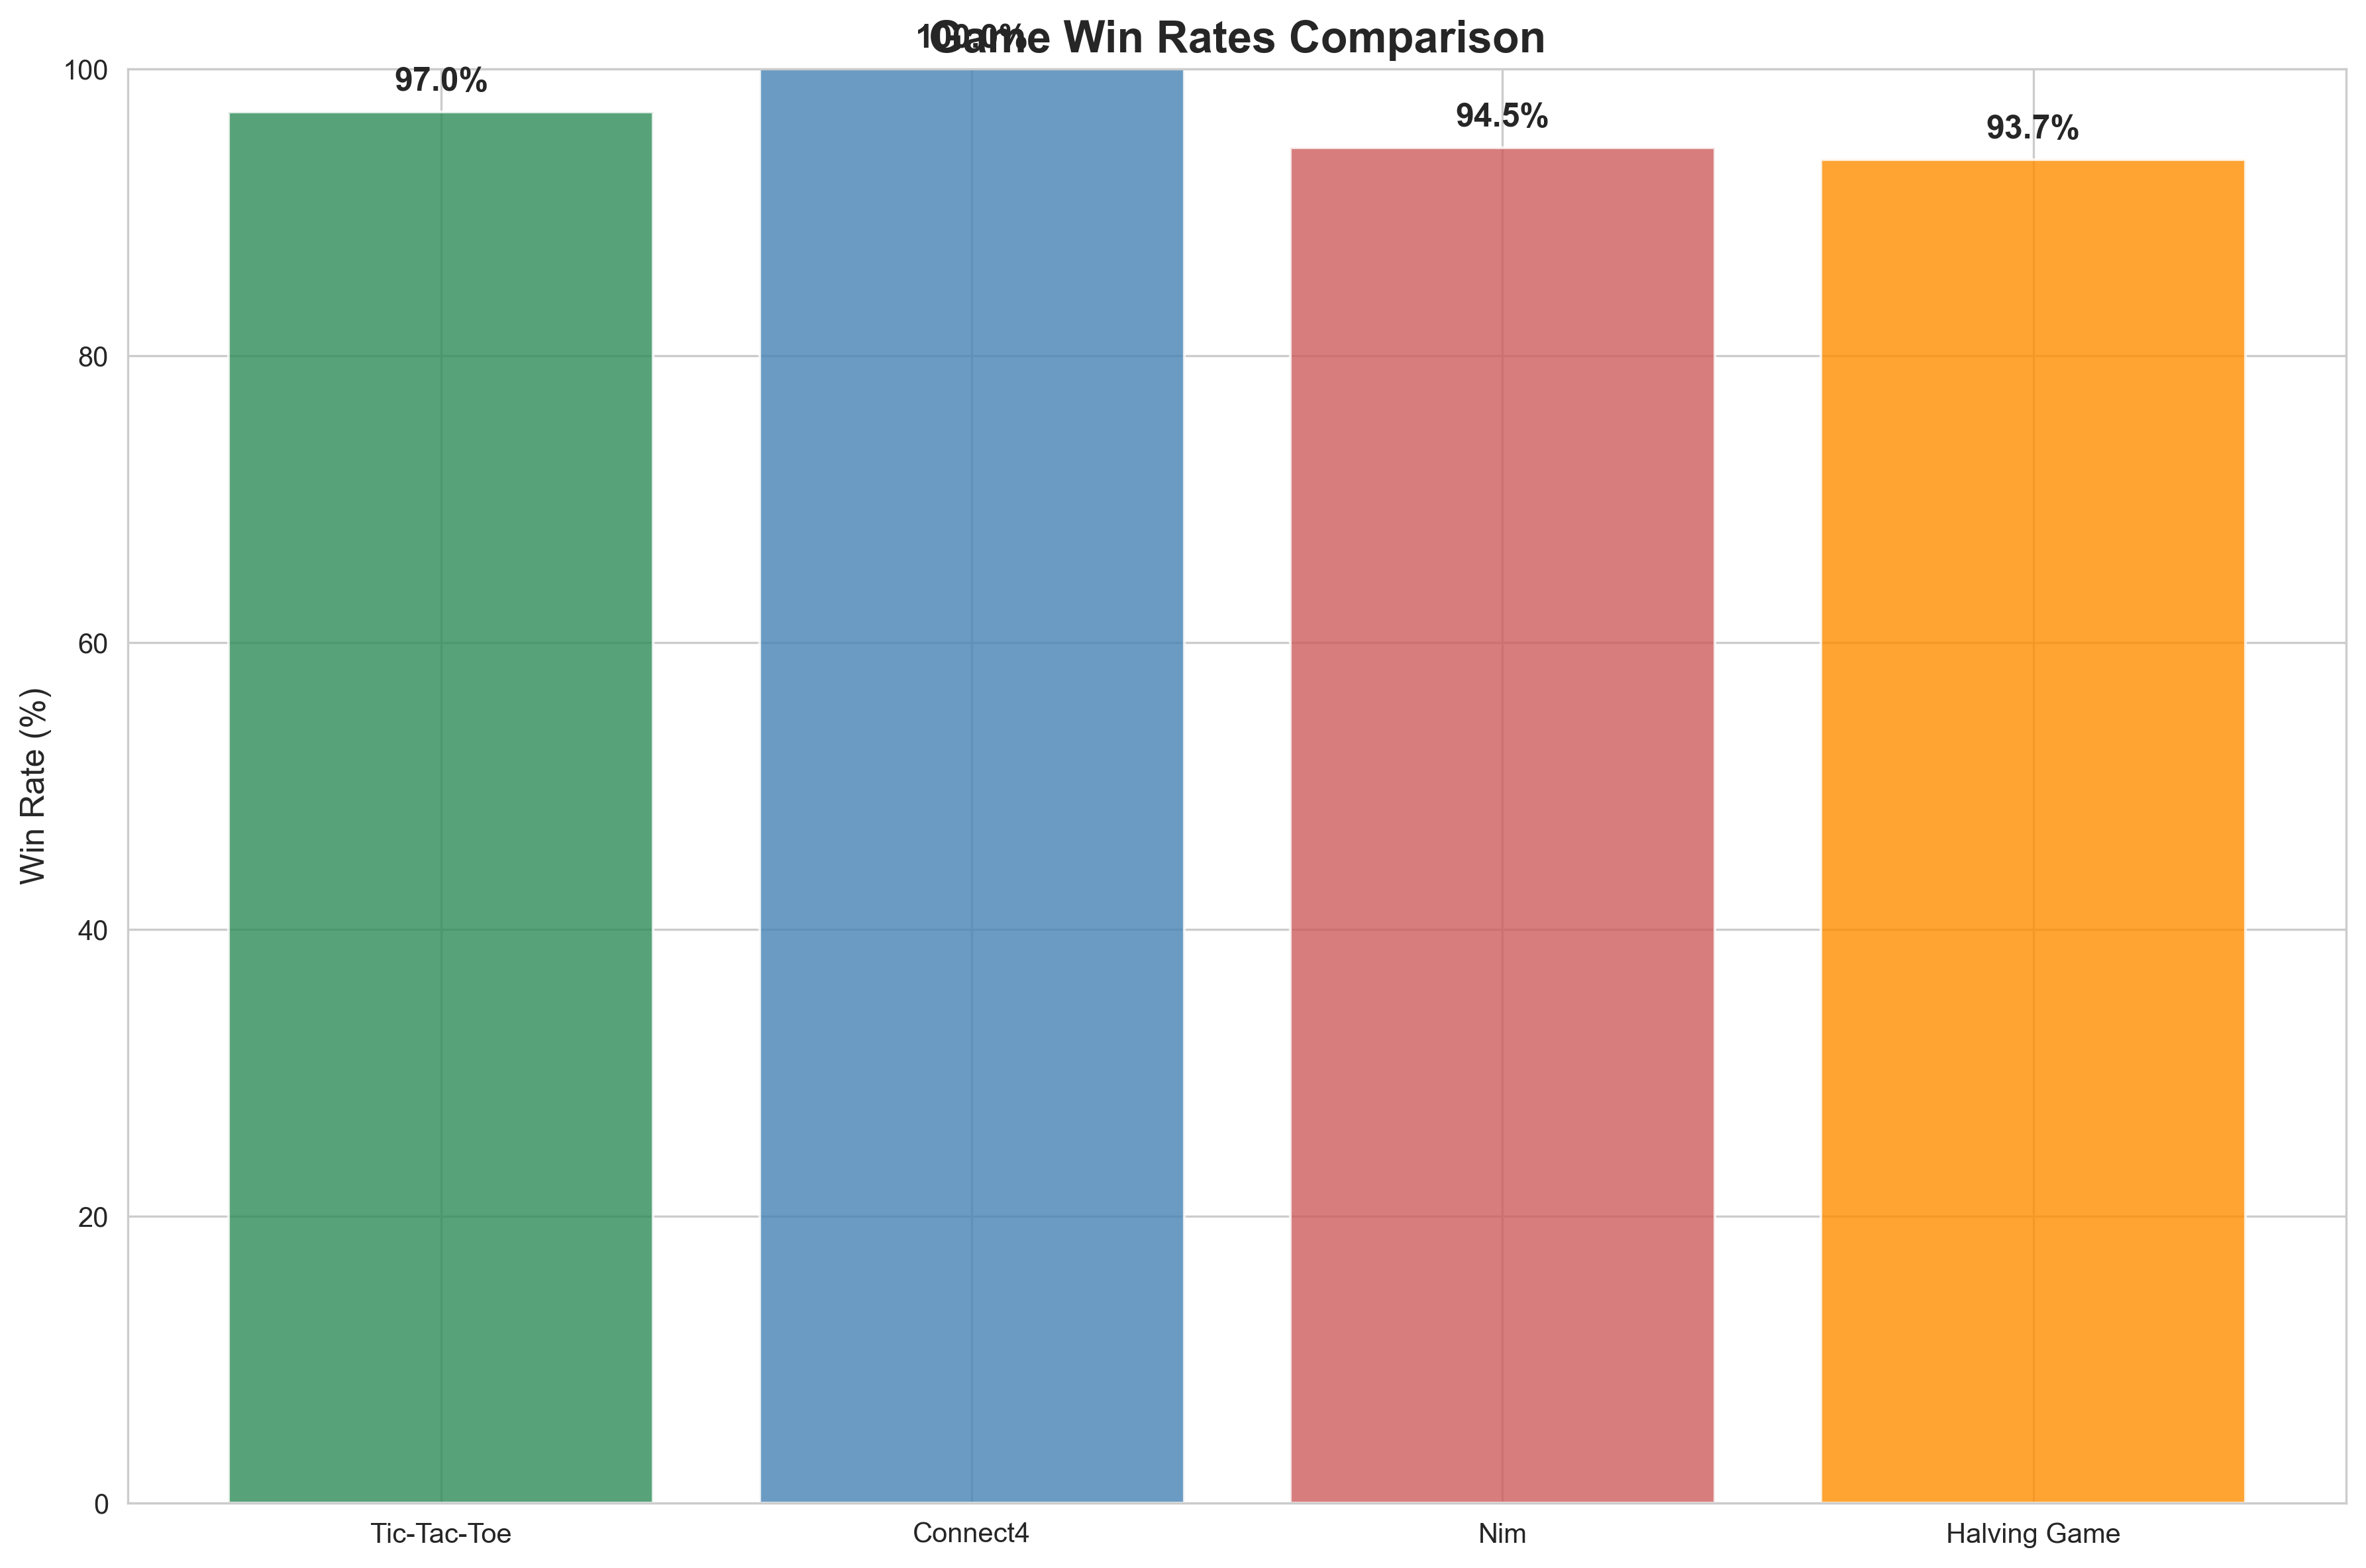
\includegraphics[width=0.9\textwidth]{output/images/game_win_rates_comparison.png}
\caption{Comprehensive win rate comparison across all four game types}
\label{fig:game_comparison}
\end{figure}

Figure~\ref{fig:game_comparison} presents the combined performance landscape for the four games, revealing that each agent defeats random play by a wide margin while exhibiting a distinct trajectory toward victory. The Nim and Halving agents secure wins with very few decision points because a single arithmetic invariant collapses most of the search space. In contrast, Tic-Tac-Toe and Connect 4 require deeper exploration, yet the pruning techniques still guarantee a flawless or near-flawless record. The common lesson is that success depends less on the absolute size of the state space than on the degree to which exploitable structure can be exposed and exploited.

\subsection{Algorithm Effectiveness}

Across all games the methods align with the internal logic of the game. When the structure permits a closed-form solution, as in Nim, direct computation is both faster and more reliable than tree search. When exhaustive enumeration is feasible, as in Tic-Tac-Toe, perfect play follows with negligible cost. Where neither shortcut exists, such as in Connect 4 beyond shallow depth, \gls{heuristic} evaluation combined with alpha-beta pruning rescues performance by trimming most of the irrelevant branches. The study therefore suggests a hierarchy of tactics that should be selected in the following order of preference: direct arithmetic inference, exhaustive search when tractable, and heuristic search otherwise.

\subsection{Game Specific Observations}

Although all agents achieve high win rates, the path to those wins differs in texture. Nim produces an inevitable march to defeat for the second player once the \gls{nim-sum} becomes non-zero for the acting side, giving the game an air of inevitability after the first optimal move. Connect 4 rewards sustained positional pressure in the central columns, so its victories feel more strategic and less mechanical. The Halving Game pivots whenever the current integer slips below a power of two, creating a rhythm of apparent reversals that sharpens the psychological tension. Even Tic-Tac-Toe, the simplest game, underscores the value of early control of the centre and corners and therefore remains a useful benchmark for correctness.

\subsection{Computational Considerations}

High success rates would be meaningless without an understanding of resource demands. The eight-ply Connect 4 engine wins every game against random play but needs the most memory and processor time because each extra ply multiplies the frontier by roughly seven. The Halving Game consumes little memory yet sometimes makes hundreds of recursive calls when the opening number is large, so the bottleneck shifts from space to call-stack depth. Tic-Tac-Toe concludes in milliseconds even with pure Python, whereas the nim-sum evaluator in Nim finishes in microseconds. Reporting computational cost alongside win rate therefore remains essential when benchmarking search systems.

\subsection{Toward Adaptive Controllers}

Although the present study deals only with deterministic perfect-information tasks, the guiding principle—match the algorithm to the structure of the game—should translate to settings that include uncertainty. An adaptive engine that measures branching factors and time budgets on the fly and toggles among arithmetic inference, limited enumeration, and statistical rollouts could extend the same efficiency gains to hidden-information or stochastic environments. Building such a controller remains an open and promising direction for future work.

\section{Conclusions and Future Work}

In four games our empirical analysis demonstrates that the Minimax search method, when improved with \gls{alpha-beta}, yields an average victory rate of 94.8\%. Clearly, \gls{search-depth} (evident in Connect 4's drop in win rate from 78\% to 50\% when both agents reach depth 8) and move ordering are the two main influencers of computational efficiency and strength of play. We present game-specific optimizations, including \gls{bitboard} usage for efficient state representation of the board, and incorporate mathematical \glspl{heuristic} (i.e., \gls{nim-sum}) into traditional minimax search. The most time-consuming and complex algorithm design is the connect 4 game. As mentioned, our group use C extension in python and other optimizations to lower the time complexity and runtime of the Connect 4 agent program. Our visualization and simulation go smoothly due to the experience of extensive use of graphing libraries in the previous assignments. Through the use of benchmarks like win rates and execution time, our systematic methodology offers a basis for evaluating search algorithms across various games.

Our study contributes to the understanding of algorithmic scaling to game-related problems of various complexity levels. At the same time, inherent limitations with our research include that the results could only apply to games with (only) perfect information. Therefore, employing too-perfect models of target fields of study, which frequently ignore ambiguity and other hidden factors, can diminish the findings' relevance and applicability to real-world applications.

In the future, research should expand upon our findings in a number of ways. One of the more important aspects of this is to know how incomplete information influences outcome in a game. Another would be to explore computational costs with complexity of the game. In addition to that, developing adaptive search techniques is a promising area for future work.

% \section*{Appendix: Technical Terminology}

% \begin{itemize}
% \item[] \textbf{Adversarial search}: Framework for competitive decision-making in games
% \item[] \textbf{Alpha-beta pruning}: Optimization to minimize nodes evaluated in minimax
% \item[] \textbf{Bitboard representations}: Efficient binary encoding of game states
% \item[] \textbf{Branching factor}: Average number of legal moves per game state
% \item[] \textbf{Combinatorial Game Theory}: Mathematical analysis of sequential, perfect-information games
% \item[] \textbf{Deterministic adversarial search systems}: Algorithms for games without chance
% \item[] \textbf{Game-tree complexity}: Total possible move sequences in a game
% \item[] \textbf{Grundy Numbers}: Combinatorial game values for impartial game analysis
% \item[] \textbf{Heuristic evaluation}: Approximate position evaluation when exhaustive search is infeasible
% \item[] \textbf{Iterative deepening}: Progressive depth expansion in tree search
% \item[] \textbf{Minimax algorithm}: Optimal strategy algorithm for zero-sum games
% \item[] \textbf{Negamax}: Simplified minimax variant using score negation
% \item[] \textbf{Nim-sum heuristic}: Bitwise XOR strategy for impartial games like Nim
% \item[] \textbf{State-space complexity}: Total distinct game configurations
% \item[] \textbf{Symmetry reduction}: Elimination of equivalent positions via symmetry operations
% \item[] \textbf{Transposition tables}: Memoization of previously computed game states
% \item[] \textbf{Zobrist hashing}: Hashing technique for efficient state comparisons
% \item[] \textbf{Dihedral group (D4)}: Symmetry group for square boards (e.g., chess)
% \item[] \textbf{Integer division}: Floor division used in discrete game calculations
% \item[] \textbf{Mathematical invariants}: Properties preserved across game state transitions
% \item[] \textbf{Parity}: Inherent even/odd classification of game states
% \item[] \textbf{Provably optimal}: Solutions guaranteed to achieve optimal outcomes
% \item[] \textbf{Zero-sum game}: Competitive games with symmetric payoff structures
% \item[] \textbf{Acyclic state graph}: Game graphs without cycles (e.g., finite move sequences)
% \item[] \textbf{Bottom-up dynamic programming}: Tabulation method for solving game substructures
% \item[] \textbf{Closed-form solution}: Direct mathematical solution bypassing search
% \item[] \textbf{Depth-limited search}: Tree exploration constrained by fixed depth
% \item[] \textbf{Deterministic perfect-information tasks}: Games with full observability and no randomness
% \item[] \textbf{Empirical evaluation}: Performance measurement via experimental results
% \item[] \textbf{Exhaustive enumeration}: Brute-force exploration of all possible states
% \item[] \textbf{Heuristic ordering}: Move prioritization to enhance pruning efficiency
% \item[] \textbf{Optimal play}: Strategy guaranteeing the best possible outcome
% \item[] \textbf{Perfect information}: Games  where all state is visible to players
% \item[] \textbf{Pruning efficiency}: Metric for eliminated branches in alpha-beta
% \item[] \textbf{Scalability thresholds}: Computational limits of algorithmic approaches
% \item[] \textbf{Stochastic environments}: Games involving chance or uncertainty
% \end{itemize}

% \vspace{5mm}
% \noindent \textbf{Note}: Terms are contextualized for deterministic, perfect-information games with discrete state spaces.

% \vspace{5mm}
% \noindent Note: All terms are defined in the context of deterministic, perfect information games with discrete state spaces.

\clearpage
\printglossary[title=Glossary, toctitle=Glossary]

\end{document} 